\documentclass{standalone}
\usepackage{times}
\usepackage{mathtools}
\usepackage{amsfonts}
\usepackage{amssymb}

\usepackage{tikz}
\usetikzlibrary{positioning,fit,shapes,calc,decorations.pathreplacing}
\usetikzlibrary{backgrounds}
\usetikzlibrary{arrows.meta}
\usetikzlibrary{shapes,snakes}

\definecolor{processblue}{cmyk}{1,1,1,0}
\definecolor{accent}{rgb}{0.0,0.5,0.8}
\definecolor{accent2}{rgb}{0.8,0.5,0.0}

\begin{document}
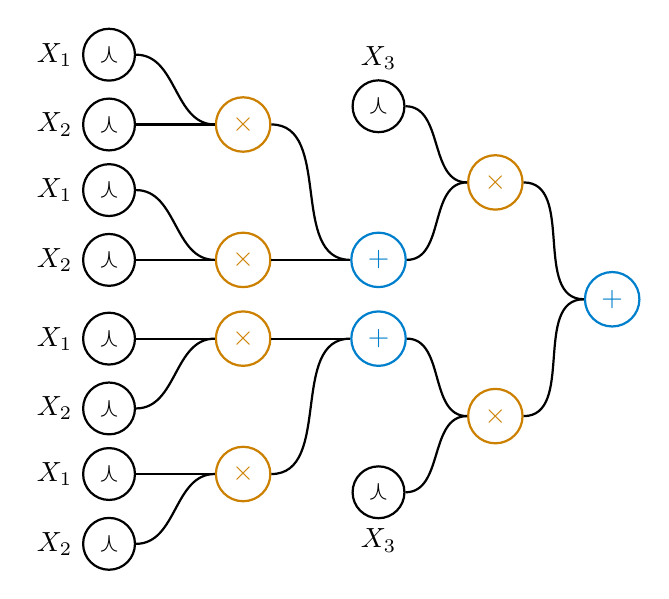
\begin{tikzpicture}[
  node/.style = {
    draw,
    circle,
    thick,
    fill = white,
    minimum width = 0.5cm,
    minimum height = 0.5cm,
  },
  >={Stealth[scale=1.8]},
]

  \node[node,draw=accent,text=accent] (root) {$+$};

  \node (d1) [left=of root] {};
  \node[node,draw=accent2,text=accent2] (p11) [above=of d1] {$\times$};
  \node[node,draw=accent2,text=accent2] (p12) [below=of d1] {$\times$};
  \path[-,thick] (p11) edge[out=0,in=180] node {} (root);
  \path[-,thick] (p12) edge[out=0,in=180] node {} (root);

  \node (d21) [left=of p11] {};
  \node[node] (p211) [above=0.5cm of d21,label={above:$X_3$}] {$\curlywedge$};
  \node[node,draw=accent,text=accent] (p212) [below=0.5cm of d21] {$+$};
  \path[-,thick] (p211) edge[out=0,in=180] node {} (p11);
  \path[-,thick] (p212) edge[out=0,in=180] node {} (p11);

  \node (d22) [left=of p12] {};
  \node[node,draw=accent,text=accent] (p221) [above=0.5cm of d22] {$+$};
  \node[node] (p222) [below=0.5cm of d22,label={below:$X_3$}] {$\curlywedge$};
  \path[-,thick] (p221) edge[out=0,in=180] node {} (p12);
  \path[-,thick] (p222) edge[out=0,in=180] node {} (p12);

  \node[node,draw=accent2,text=accent2] (p312) [left=of p212] {$\times$};
  \node[node,draw=accent2,text=accent2] (p311) [above=of p312] {$\times$};
  \path[-,thick] (p311) edge[out=0,in=180] node {} (p212);
  \path[-,thick] (p312) edge[out=0,in=180] node {} (p212);

  \node[node,draw=accent2,text=accent2] (p321) [left=of p221] {$\times$};
  \node[node,draw=accent2,text=accent2] (p322) [below=of p321] {$\times$};
  \path[-,thick] (p321) edge[out=0,in=180] node {} (p221);
  \path[-,thick] (p322) edge[out=0,in=180] node {} (p221);

  \node[node] (p412) [left=of p311,label={left:$X_2$}] {$\curlywedge$};
  \node[node] (p411) [above=0.2cm of p412,label={left:$X_1$}] {$\curlywedge$};
  \path[-,thick] (p411) edge[out=0,in=180] node {} (p311);
  \path[-,thick] (p412) edge[out=0,in=180] node {} (p311);

  \node[node] (p422) [left=of p312,label={left:$X_2$}] {$\curlywedge$};
  \node[node] (p421) [above=0.2cm of p422,label={left:$X_1$}] {$\curlywedge$};
  \path[-,thick] (p421) edge[out=0,in=180] node {} (p312);
  \path[-,thick] (p422) edge[out=0,in=180] node {} (p312);

  \node[node] (p431) [left=of p321,label={left:$X_1$}] {$\curlywedge$};
  \node[node] (p432) [below=0.2cm of p431,label={left:$X_2$}] {$\curlywedge$};
  \path[-,thick] (p431) edge[out=0,in=180] node {} (p321);
  \path[-,thick] (p432) edge[out=0,in=180] node {} (p321);

  \node[node] (p441) [left=of p322,label={left:$X_1$}] {$\curlywedge$};
  \node[node] (p442) [below=0.2cm of p441,label={left:$X_2$}] {$\curlywedge$};
  \path[-,thick] (p441) edge[out=0,in=180] node {} (p322);
  \path[-,thick] (p442) edge[out=0,in=180] node {} (p322);
\end{tikzpicture}
\end{document}
